\section{Admission-benchmarks/Grade \% Correlation}
Correlation coefficients ($r$) between different admissions benchmarking methods and CSC1015F course results are worked out for students that are South African citizens or permanent residents, and that attended CSC1015F during their undergraduate career. correlation is worked out on retrieval of the dataset comprising a join of admissions and grade data. In terms of SQL, such a join can be described as a \textit{left outer join} in which rows of the benchmark data are joined to rows of the grade data on the student number field; a single student may have many grade results (for example, when repeating a course) but only has a single row in the admissions data for the year in which the student first registered.

\subsection{ETL}
Using nETL, rows are extracted from the two CSV files (\textit{Admissions (2014 - 2016).csv} and \textit{Grades (2014 - 2016).csv}) independently of each other and concurrently, in batches of 5 000 and 10 000 rows respectively.

Via nETL configuration, rows from the admissions data are selected for students that are South African citizens or permanents residents, and that are in undergraduate; rows from the grades data are selected for students that attended CSC1015F during their undergraduate career. A dynamic filter is applied to the admissions data to further select only students that attended CSC1015F.

Batches of data from both CSVs is loaded into a single CouchDB database via the \textit{\_bulk\_docs} endpoint. A list of the transformations applied to each line extracted from each CSV is shown below:

\subsubsection{nETL Grades Transformations}
\begin{enumerate}
  \item A line is converted into a JavaScript object (which relates directly to the JSON format of CouchDB documents) with the fields:
        \begin{itemize}
          \item DownloadedDate
          \item RegAcadYear
          \item RegTerm
          \item anonIDnew
          \item RegProgram
          \item RegCareer
          \item Degree
          \item DegreeDescr
          \item Subject
          \item Catalog.
          \item Course
          \item CourseSuffix
          \item Session
          \item Percent
          \item Symbol
          \item UnitsTaken
          \item CourseID
          \item CourseDescr
          \item CourseCareer
          \item Faculty
          \item Dept
          \item MaximumCrseUnits
          \item CourseCount
          \item CourseLevel
          \item CESM
          \item Sub-CESM
        \end{itemize}
  \item Lines (now in object form) are filtered on the ``RegCareer'' and ``Course'' fields, where grades achieved for the CSC1015F course taken by students registered as undergrads are considered. Lines that don't meet this attribute are discarded and no further transformations are applied to these line
  \item An attribute (``type\_'') is then added to each line (that weren't removed in filtering step), and given the value ``grade'' to identify each object as a line of the Grade entity type
  \item Document attributes are whitelisted. The resultant documents each have the the following attributes:
        \begin{itemize}
          \item type\_
          \item Course
          \item RegAcadYear
          \item anonIDnew
          \item Percent
        \end{itemize}
\end{enumerate}

\subsubsection{nETL Benchmarks Transformations}
\begin{enumerate}
  \item A line is converted into a JavaScript object with the fields:
        \begin{itemize}
          \item anonIDnew
          \item Career
          \item Citizenship Residency
          \item SA School
          \item Eng Grd12 Fin Rslt
          \item Math Grd12 Fin Rslt
          \item Mth Lit Grd12 Fin Rslt
          \item Adv Mth Grd12 Fin Rslt
          \item Phy Sci Grd12 Fin Rslt
          \item NBT AL Score
          \item NBT QL Score
          \item NBT Math Score
          \item RegAcadYear
        \end{itemize}
  \item Lines are filtered on the ``Career'', ``Citizenship Residency'', and ``anonIDnew'' fields. Only lines for students that attended the CSC1015F course during their undergraduate career and that are either South African citizens or permanent residents are included in the result set. The list of students that attended CSC1015 is derived from the Grade data
  \item An attribute (``type\_'') is then added to each remaining line and given the value ``benchmark'' to identify each object as a line of the Benchmark entity type
  \item Attributes are whitelisted. The resultant documents each have the the following attributes:
        \begin{itemize}
          \item type\_
          \item anonIDnew
          \item Eng Grd12 Fin Rslt
          \item Math Grd12 Fin Rslt
          \item Mth Lit Grd12 Fin Rslt
          \item Adv Mth Grd12 Fin Rslt
          \item Phy Sci Grd12 Fin Rslt
          \item NBT AL Score
          \item NBT QL Score
          \item NBT Math Score
          \item RegAcadYear
        \end{itemize}
\end{enumerate}

\subsection{MapReduce}
Following loading the data from the CSVs into CouchDB, a Map function is used to produce an index of the CouchDB documents ordered by Student ID, with the guarantee that for every unique student id documents are ordered by type; the demographic document precedes the Grade documents for any given student. Knowing the order of documents via the view-index allows for performing the join on data-retrieval. Only a map function is used is required (no reduce function). Each document passed to the map function is treated according to the logic shown in the activity diagram in Figure \ref{fig-2-way-join-map-function}. That is, on Map function execution the ``type\_'' attribute is checked. If the document is a line of the Grades entity, then the key [Student ID, Course, year] is emitted along with a single number for the value - the percent achieved for the course. If the document is a line of the Benchmarks entity, then the key [student ID, 0, 0] is emitted along with an ordered list of 8 values corresponding to the different benchmarks:

\begin{itemize}
  \item Gr12 English \%
  \item Gr12 science \%
  \item Gr12 Math \%
  \item Gr 12 Math Lit \%
  \item Gr12 Adv Math \%
  \item NBT AL \%
  \item NBT QL \%
  \item NBT Math \%
\end{itemize}

Normalization of the percentage fields (i.e. ``Percent'' for the Grades entity and the test results in the Benchmarks entity) is done via a nested function within the Map function as discussed previously (Table \ref{tbl-grades-normalize} and Table \ref{tbl-benchmarks-normalize}). No reduce function is used to achieve this 2-way join. This is because, theoretically, a student should only have a single set of Benchmark results and should only achieve a single grade per course per year. As such there is no need to aggregate output from the Map function (which is done via reduction) before performing the document join via the List function.

\begin{figure}[H]
    \centering
    \begin{mdframed}
        \centering
        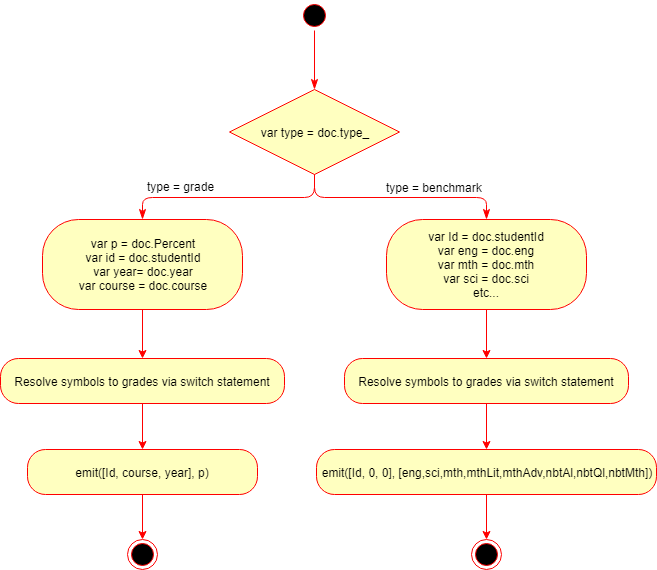
\includegraphics[scale=0.59]{./resources/figures/2-way-join-map.png}
    \end{mdframed}
    \caption[2-Way Join Map Function]{\textbf{Figure \ref{fig-2-way-join-map-function}: 2-way join \textit{map} function logic}
    \label{fig-2-way-join-map-function}
\end{figure}


\subsection{List Function: calculating correlation}
The list function is executed via a call to CouchDB's HTTP API. For the project the URI of that function call is \url{https://localhost:5984/msc/\_design/2-way-join/\_list/2-way-join-list/ 2-way-join-view?reduce=false}. On invocation the List function opens and scans the index iteratively processing each document (i.e. iteratively processing each student; first a student's demographic document is processed, then a student's grades documents are processed). The join is performed during list function execution alongside calculation of correlation coefficients according to the formula \footnote{Unlike when working out variance of a dataset, summation is handled manually in this case.} \footnote{\textit{x}: grade \%, \textit{y}: benchmark (\textit{r} is calculated for multiple \textit{y} values)}: \begin{spreadlines}{15pt}
  \begin{gather*}
    \intertext{\textit{Pearson Correlation Coefficient:}}
    r = \frac{N\sum{xy} - (\sum{x})(\sum{y})}{\sqrt{[N\sum{x^2} - (\sum{x})^2][N\sum{y^2} - (\sum{y})^2]}}
  \end{gather*}
\end{spreadlines}

When calculating variance (as shown previously), only a single data entity was used. As such the \_stats function could be used as a means of creating aggregations for corresponding values such as \textit{sum of squares}, \textit{sum} and \textit{count}, and then variance could be worked out in reference to these aggregated values. Working out correlation cannot make use of CouchDB's \_stats reduce function, since entities are reduced separately and only final aggregations of each entity are made available on data retrieval. For example, in reference to working out the numerator in reference to correlation: \begin{spreadlines}{15pt}
  \begin{gather*}
    N\sum{xy} - (\sum{x})(\sum{y})
  \end{gather*}
\end{spreadlines}

Using CouchDB's \_stats function only the $\sum{x}$ and $\sum{y}$ values are accessible when joining the two entities during list function execution, and not $x$ and $y$ values (similarly, the denominator of the formula could also not be calculated from \_stats function output). As such, to work out the correlation between grades and benchmarks requires aggregations across entities during list function execution; essentially the list function is used to aggregate numerical data from disparate entities by means of join which is performed iteratively per student number. To achieve this, the list function is required to work with running totals as the index (the output of the map function without using a reduce function) is iterated over.





Figure \ref{fig-2-way-join-list-function} shows an activity digram representing the logic used to perform the 2-way join in the List function. The logic is wrapped in a CouchDB helper function \mintinline{text}{provides()} that accepts two arguments: the type of data the list function will emit (CSV - i.e. plain text data), and a callback that allows uses to create the data that is transformed to the output type. Within the body of the callback the variables `currentStudent', `currentYear', and `currentLine' are set to null. An iteration over the index is initiated using a while loop, with the loop invariant the result of a call to the \textit{getRow()} function. When a row exists, a check is performed on whether the Student ID of the current row is the same as the Student ID of the previous row. If not, the currentLine variable is emitted via the \textit{send()} function, and currentStudent is adjusted to be the Student ID from the current row. Then the type of row being processed is checked (i.e. whether this key:value pair was emitted from a grade or benchmark document). If from a benchmark document, the scores are added to the currentLine variable and the loop re-executes. If a Grade document, there is a check as to whether \textit{currentYear} has the same value as the Year property in the current row. If not, the \textit{currentLine} variable is emitted and \textit{currentYear} is adjusted to the new Year value and the loop re-executes. When the loop invariant becomes false the subroutine to send the currentLine is executed one last time to take into account the last document processed. \textit{currentLine} is emitted via a subroutine which first checks that the currentLine variable contains data from both the Grades and Benchmarks entity, and if not the line is discarded. Otherwise \textit{send()} is called with a comma-delimited string as a parameter, and this is emitted as output via a stay-alive network request (the connection is handled by the HTTP client).

\begin{figure}[H]
    \centering
    \begin{mdframed}
        \centering
        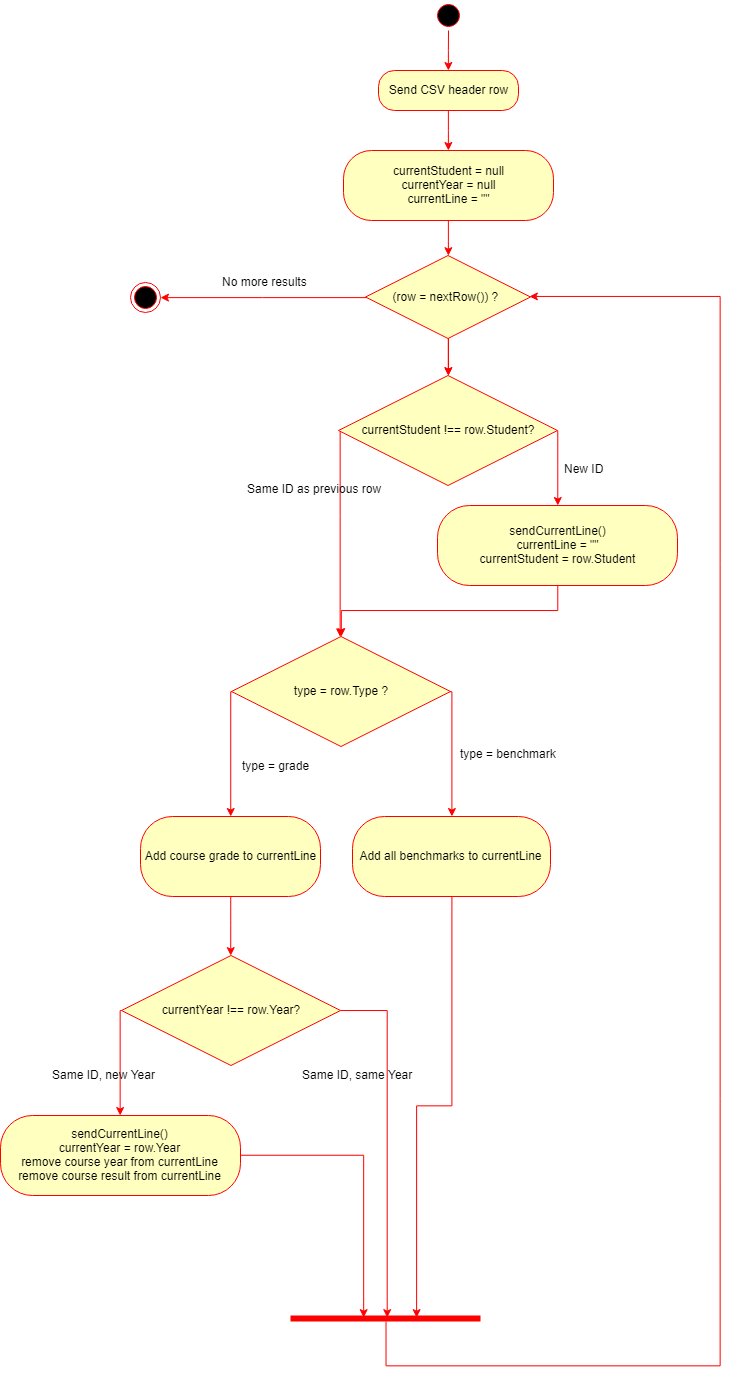
\includegraphics[scale=0.5]{./resources/figures/2-way-join-list.png}
    \end{mdframed}
    \caption[2-Way Join List Function]{\textbf{Figure \ref{fig-2-way-join-list-function}: List function logic required to join the Grades and Benchmarks entities.} Activity diagram of the code executed within the callback passed to the provides function executed by CouchDB during runtime of List function.}
    \label{fig-2-way-join-list-function}
\end{figure}


\subsection{Output}
A sample of the resultant joined dataset is shown in Figure \ref{fig-2-way-csv-output}. The full output has 1391 rows; 350 rows for the 2014 year, 457 rows for the 2015 year, 586 rows for the 2016 year. Many student IDs are repeated for different years; this occurs when students retake the course in a subsequent year. In this case, due to the nature of the sorted view index from CouchDB, all a student's course attempts are seen as separate, sequential rows in the joined output.

\begin{sidewaysfigure}
    \centering
    \begin{mdframed}[rightline=false,topline=false,leftline=false]
        \centering
        \begin{BVerbatim}
+------+---------+----------+-------+---------+---------+---------+-------------+-------------+-------+-------+--------+
| Year |   ID    |  Course  | Grade | G12 Eng | G12 Sci | G12 Mth | G12 Mth Lit | G12 Mth Adv | NBTAL | NBTQL | NBTMth |
+------+---------+----------+-------+---------+---------+---------+-------------+-------------+-------+-------+--------+
| 2015 | 2749802 | CSC1015F |    71 |      79 |      72 |      85 |           0 |           0 |    86 |    94 |     91 |
| 2015 | 2794606 | CSC1015F |    77 |      75 |      84 |      78 |           0 |           0 |     0 |     0 |      0 |
| 2014 | 2854832 | CSC1015F |    87 |      88 |       0 |      97 |           0 |           0 |    81 |    83 |     82 |
| 2014 | 2860166 | CSC1015F |    37 |       0 |       0 |       0 |           0 |           0 |     0 |     0 |      0 |
| 2016 | 2862568 | CSC1015F |    63 |      80 |       0 |      95 |           0 |           0 |    78 |    79 |     82 |
| 2014 | 2863288 | CSC1015F |    81 |      86 |       0 |      93 |           0 |           0 |    82 |    86 |     90 |
| 2015 | 2863336 | CSC1015F |    66 |      71 |      74 |      75 |           0 |           0 |    76 |    78 |     66 |
| 2015 | 2864266 | CSC1015F |    49 |      55 |       0 |      74 |           0 |           0 |    59 |    66 |     61 |
| 2016 | 2864266 | CSC1015F |    64 |      55 |       0 |      74 |           0 |           0 |    59 |    66 |     61 |
| 2014 | 2880284 | CSC1015F |    64 |      68 |       0 |      93 |           0 |           0 |    65 |    92 |     78 |
| 2014 | 2881364 | CSC1015F |    68 |      87 |       0 |      84 |           0 |           0 |    81 |    86 |     73 |
| 2014 | 2882706 | CSC1015F |    85 |      82 |       0 |      97 |           0 |           0 |    83 |    83 |     92 |
| 2014 | 2890964 | CSC1015F |    80 |      74 |       0 |      88 |           0 |           0 |    78 |    88 |     71 |
| 2014 | 2894402 | CSC1015F |    78 |      70 |       0 |      86 |           0 |           0 |    66 |    71 |     70 |
| 2014 | 2894954 | CSC1015F |    87 |      72 |       0 |      94 |           0 |           0 |    81 |    93 |     88 |
| 2014 | 2895244 | CSC1015F |    64 |      77 |       0 |      85 |           0 |           0 |    72 |    54 |     45 |
| 2015 | 2896964 | CSC1015F |    76 |      77 |       0 |      84 |           0 |           0 |    66 |    82 |     71 |
+------+---------+----------+-------+---------+---------+---------+-------------+-------------+-------+-------+--------+
        \end{BVerbatim}
    \end{mdframed}
    \caption[Sample of 2-way CSV output]{\textbf{Figure \ref{fig-2-way-csv-output}: Sample of the 2-way join output CSV.} List function output is a CSV download with the schema as represented in this figure. The full CSV has 1391 rows; 350 rows for the 2014 year, 457 rows for the 2015 year, 586 rows for the 2016 year. Many student IDs are repeated for different years; this occurs when students retake the course in a subsequent year. In this case, due to the nature of the sorted view index from CouchDB, all a student's course attempts are sequential rows.}
    \label{fig-2-way-csv-output}
\end{sidewaysfigure}
